\documentclass[fleqn]{article}
\usepackage{accsupp}
\usepackage{amssymb}
\usepackage{mathtools}
\usepackage{geometry}
\usepackage{graphics}
\usepackage[utf8]{inputenc} 
\usepackage[english]{babel}
\usepackage{tabularx}
\usepackage{lastpage}
\usepackage{listings}
\usepackage{xcolor}
\usepackage{courier}
\usepackage{url}
\geometry{
	a4paper,
	total={170mm,257mm},
	left=20mm,
	top=20mm,
}
\usepackage{fancyhdr}
\setlength{\headsep}{0pt}
\pagestyle{fancy} 
\rfoot{\thepage\ of \pageref{LastPage}}
\lfoot{Rover documentation: camera stream and browser control}
\cfoot{}
\renewcommand{\footrulewidth}{1pt}

\lstset{language=C, numbers=left, numberstyle=\small, basicstyle=\ttfamily\bfseries, showstringspaces=false, numbersep=10pt, numberblanklines=false, frame=single,  backgroundcolor=\color{mygray}, xleftmargin=15pt,  linewidth=1\linewidth,  breaklines=true, captionpos=b, tabsize=2, keywordstyle=\bfseries, morekeywords={package, class, final, new, WHILE, ENDWHILE, FOR, ENDFOR, IF, ENDIF, ELSE, SWITCH, CASE, ENDSWITCH}, escapeinside={*@}{@*}, breakindent=5pt}
%commentstyle=\color{olive},
\definecolor{mygray}{gray}{.95}

\begin{document}
	\title{\rule{\textwidth}{1pt}\textbf{ Rover Documentation} \\ Browser-based Camera Stream \& Drive Control \rule{\textwidth}{1pt}\vspace{-20pt}}
	\date{}
	%\author{Dortmund University of Applied Sciences and Arts\\ IDiAL institute \\APP4MC Rover}
	\maketitle 
	\setlength{\headsep}{20pt}
	\vspace{-20pt}
	\begin{tabularx}{\textwidth}{Xlll}
		& \textit{Version} & \textit{\today }&\\
		&\textit{Implementation} &\textit{Mustafa Özcelikörs} & \textit{mozcelikors@gmail.com}\\
		&\textit{Supervision \& revision} &\textit{Robert Höttger} &\textit{robert.hoettger@fh-dortmund.de}\\ \\
		&&\multicolumn{2}{l}{University of Applied Sciences and Arts Dortmund}\\ 
		&&\multicolumn{2}{l}{IDiAL Institute, Project AMALTHEA4public}\\
		&&\multicolumn{2}{l}{BMBF  	Fund.Nb. 01|S14029K} 
	\end{tabularx} 
	\vspace{15pt}\\
	\begin{tabularx}{\textwidth}{cXc}
		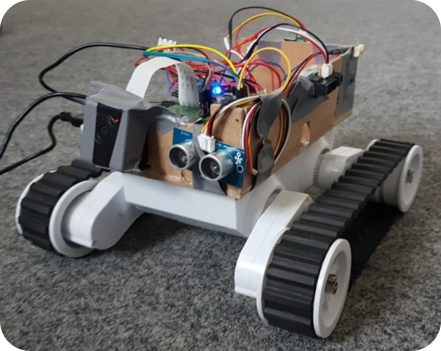
\includegraphics{rover.png} & &	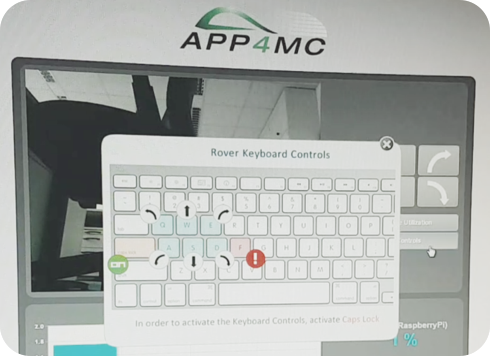
\includegraphics{page.png}\\
	\end{tabularx}
	\section{General structure}
	\begin{figure}[h!]
	\centering
	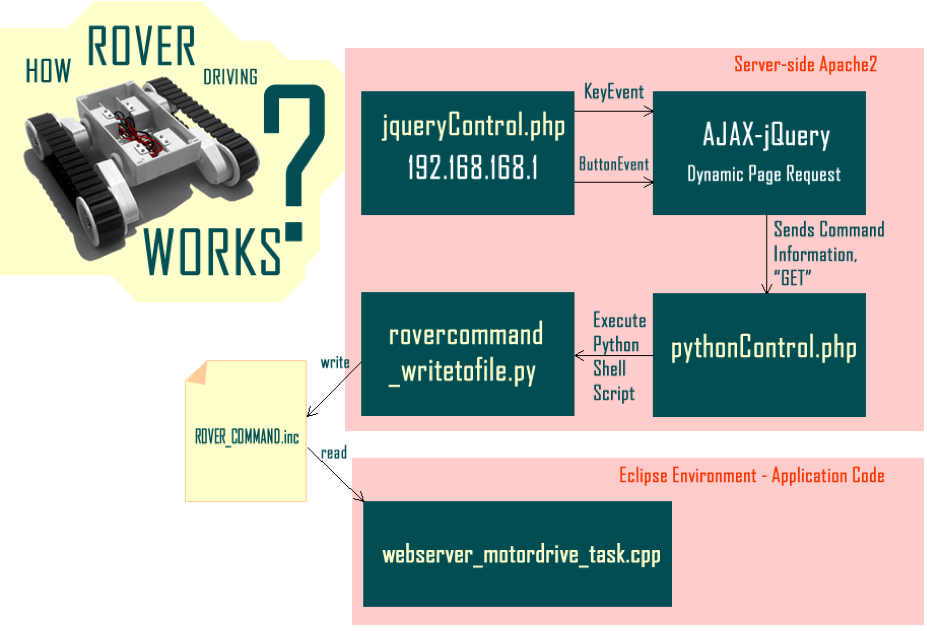
\includegraphics[width=0.7\textwidth]{structure.png}
	\caption{General structure of this documentation's rover control}
	\label{fig:struct}
	\end{figure}

	\section{Introduction}
The script provided does not require extra configuration to setup IP addresses, which are dynamically obtained. The only requisite is connecting to the same IP address via the following in your browser:
\begin{lstlisting}[label={lst:1}]
http:*@//@*<Your_IP_Address>/jqueryControl.php
\end{lstlisting}
If your rover provides the hotspot from PolarSys, use
\begin{lstlisting}[label={lst:partWrkflw}]
http:*@//@*192.168.168.1/jqueryControl.php
\end{lstlisting}

	\section{Apache2 and PHP5 Installation and Configuration}
	In order to start driving the rover from a web page, one should install Apache2 and PHP5. To get the latest packages from the repository list go into shell and type (\textit{internet connectivity required}):
\begin{lstlisting}
sudo apt-get update
sudo apt-get upgrade
\end{lstlisting}
To install apache2 type:
\begin{lstlisting}
sudo apt-get install apache2 -y
sudo apt-get install php5 libapache2-mod-php5 -y
\end{lstlisting}
Afterwards, the webpage should be located at \texttt{/var/www/html} directory. In order to give certain permissions to the current user execute: 
\begin{lstlisting}
sudo chgrp -R www-data /var/www/html
sudo find /var/www/html -type d -exec chmod g+rx {} +
sudo find /var/www/html -type f -exec chmod g+r {} +
\end{lstlisting}
In the following, replace USER with your user name, which is typically "pi" in Raspbian:

\begin{lstlisting}
sudo chown -R USER /var/www/html/
sudo find /var/www/html -type d -exec chmod u+rwx {} +
sudo find /var/www/html -type f -exec chmod u+rw {} +
\end{lstlisting}
Subsequently, enable access to the Linux file-system from the provided webpage via:
\begin{lstlisting}
sudo visudo
\end{lstlisting}
Within the editor, add the following to the end, save the file, and exit (depending on your default editor)
(Saving and exiting in Nano editor $Ctrl+O \rightarrow Y \rightarrow Enter$, saving and exiting in Emacs editor $Ctrl + X \rightarrow Ctrl + S \rightarrow Enter \rightarrow Ctrl + X \rightarrow K \rightarrow Enter$) 
\begin{lstlisting}
www-data ALL=(ALL) NOPASSWD: ALL
\end{lstlisting}
\section{Setting up the webpage}
After the RPI setup is complete, move the provided webpage zip file to the web server folder,extract it, and delete the zip via:
\begin{lstlisting}
sudo mv /home/pi/Downloads/RoverWebpage_FHDO.zip /var/www/
cd /var/www/ 
sudo unzip RoverWebpage_FHDO.zip
sudo rm -rf RoverWebpage_FHDO.zip
\end{lstlisting}
\section{Installing psutil}
In order to monitor core utilization, a python pip package called 'psutil' needs to be installed:
\begin{lstlisting}
sudo apt-get install python-dev python3-dev
cd /var/www/html/
sudo pip install psutil/
\end{lstlisting}
\section{Installing Raspberry Pi Camera and Streamer}
\textit{Note: The following parts are quite error prone. Please contact us if you have problems.}
Firstly, install the Raspberry Pi camera via:
\begin{lstlisting}
sudo raspi config
\end{lstlisting}
Select Advanced $\rightarrow$ Enable Camera, and then save and reboot your Pi.Installation of the Streamer requires a .so specific file input\_raspicam.so if you are using Raspicam instead of a webcam. This is provided with the .zip file, but needs to be installed properly. Now, we should first clean up the build:
\begin{lstlisting}
cd /var/www/html/camerastuff/newmjpg-streamer/mjpg-streamer/mjpg-streamer-experimental
sudo make clean
\end{lstlisting}
Afterwards, clean up the CMAKE cache and install via:
\begin{lstlisting}
sudo rm -rf CMakeCache.txt
sudo cmake
sudo make
sudo make install
\end{lstlisting}
Copy the necessary libraries and executables in the respective folders:
\begin{lstlisting}
sudo cp mjpg_streamer /usr/local/bin
sudo cp output_http.so input_raspicam.so input_uvc.so /usr/local/lib/
\end{lstlisting}
Before testing the camera,  permissions to the executables and libraries have to be set:
\begin{lstlisting}
sudo chmod 777 /usr/local/lib/*.so
sudo chmod 777 /usr/local/bin/mjpg_streamer
\end{lstlisting}
Finally, the camera can be tested. With the following command (if there are no errors)the setup should be working. The following not only makes the executables know the location of the libraries but also sets up a reliable and fast input connection for raspberry pi camera:
\begin{lstlisting}
sudo bash /var/www/html/camerastuff/webcam_stream_start_from_rpi_camera.bash
\end{lstlisting}
The following provides the specific content of this file, that can be adjusted towards specific needs:
\begin{lstlisting}
#!/bin/bash
sudo bash /var/www/html/camerastuff/newmjpg-streamer/mjpg-streamer/mjpg-streamer-experimental 
export LD_LIBRARY_PATH=/usr/local/lib
sudo /usr/local/bin/mjpg_streamer -i "/usr/local/lib/input_raspicam.so -x 640 -y 480 -fps 30" -o "/usr/local/lib/output_http.so -w /usr/local/www -p 8081"
\end{lstlisting}
After starting this .bash file, the webpage at \url{http://192.168.168.1/jqueryControl.php} should show the camera stream.
\newpage
\section{Adjustments to the rover application}
Since the rover does not yet consider the webpage commands,the rover control application code must be edited. To do so, find the newest version of the Eclipse application, which contains necessary adjustments and include the following task function:
\begin{lstlisting}
void *WebServer_MotorDrive_Task(void * arg)
{
	FILE *fp;
	char ch;

	while(1)
	{
		fp = fopen("/var/www/html/ROVER_CMD.inc", "r");
		ch = fgetc (fp);
		//printf("Got command = %c\n", ch);
		pthread_mutex_lock(&keycommand_lock);
		keycommand_shared = tolower(ch);
		pthread_mutex_unlock(&keycommand_lock);
		fclose(fp);
		delayMicroseconds(50000);//50ms
	}
}
\end{lstlisting}
\section{Completion}
In order to be able to use the web-page with its all functions, the following commands have to be executed on the rover before connecting to the webpage after a reboot.
\begin{lstlisting}
sudo python /var/www/html/initialize.py
sudo bash /var/www/html/camerastuff/ webcam_stream_start_from_rpi_camera.sh  &
sudo python /var/www/html/record_core_usage_rpi.py
\end{lstlisting}
To make everything permanent, it is suggested to put the following into a/etc/rc.local file. Before exit 0 command in /etc/rc.local/, add:
\begin{lstlisting}
cd /var/www/html/
sudo python /var/www/html/initialize.py &
sudo python /var/www/html/record_core_usage_rpi.py &
sudo bash /var/www/html/camerastuff/webcam_stream_start_from_rpi_camera.sh  &
\end{lstlisting}
\end{document}